\documentclass[11pt,a4paper]{article}

\usepackage{amsmath}
\usepackage{graphicx}
\usepackage{epstopdf}

\title{AMTH250 \\ Assignment 7}

\author{Mark Villar}

\begin{document}

\maketitle

\subsubsection*{Question 1} 
$$f(x)=\sin(10x)-x, \ x \in [-1,1]$$
\begin{center}
	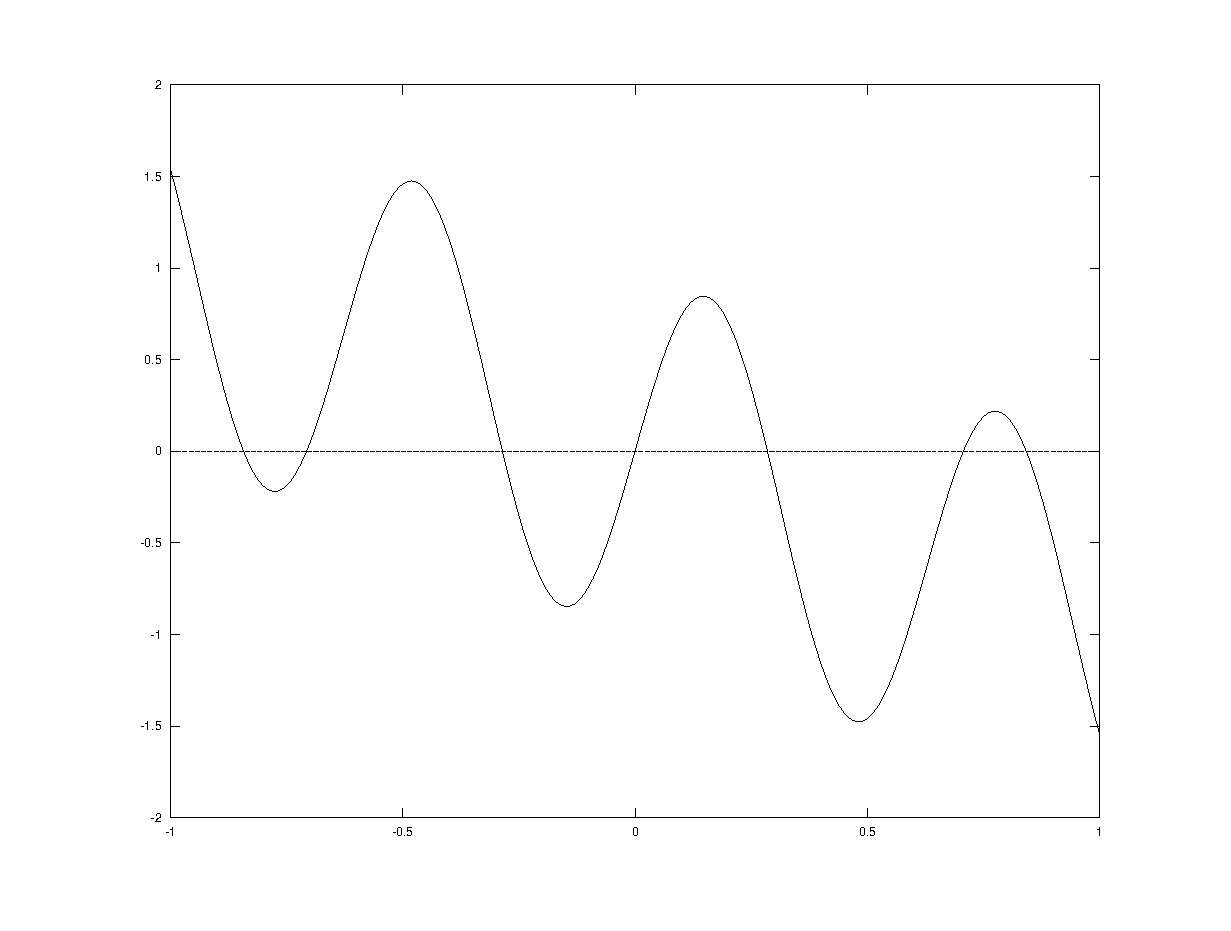
\includegraphics[width=0.9\textwidth]{wave.eps}
\end{center}
The zeros of the function are $\pm0.28523, \pm0.70682, \pm0.84232$ and 0.

\subsubsection*{Question 2}
We plot $y=x$ and $y=\tan(x)$ and deduce that the curves will intersect for the millionth time in the interval $\big[1000000\pi,\frac{2000001}{2}\pi \big]$. Applying the fzero command to the function $f(x)=x-\tan(x)$, we obtain 
$$x_{1000000}\approx 3141594.22438580$$

\subsubsection*{Question 3}
\begin{enumerate}
	\item[(a)]
	\begin{enumerate}
		\item[(i)] $g_1(x)=(x^2+2)/3$ \\
		$g_1'(x)=2x/3 \ \Rightarrow \ g_1'(2)=4/3$ \ (divergent)
		\item[(ii)] $g_2=\sqrt{3x-2}$ \\
		$g_2'(x)=\dfrac{3}{2\sqrt{3x-2}} \ \Rightarrow \ g_2'(2)=3/4$ \ (linearly convergent)
		\item[(iii)] $g_3=3-2/x$ \\
		$g_3'(x)=2/x^2 \ \Rightarrow \ g_3'(2)=1/2$ \ (linearly convergent)
		\item[(iv)] $g_4=(x^2-2)/(2x-3)$ \\
		$g_4'(x)=\dfrac{2(x^2-3x+2)}{(3-2x)^2} \ \Rightarrow \ g_4'(2)=0$ \ (quadratically convergent)
	\end{enumerate}
	\item[(b)]
	\begin{enumerate}
		\item[(i)] This fixed point iteration fails to converge at $x=2$. \\
		For $x(0)<2$, convergence does occur but at the other root, $x=1$.
		\begin{verbatim}
		x1 =
		Columns 1 through 7:
		1.9000   1.8700   1.8323   1.7858   1.7297   1.6639   1.5895

		Columns 8 through 14:
		1.5089   1.4256   1.3441   1.2688   1.2033   1.1493   1.1070
		
		Columns 15 through 21:
		1.0751   1.0520   1.0356   1.0241   1.0163   1.0109   1.0073
		
		Columns 22 through 28:
		1.0049   1.0033   1.0022   1.0015   1.0010   1.0007   1.0004
		
		Columns 29 through 35:
		1.0003   1.0002   1.0001   1.0001   1.0001   1.0000   1.0000
		\end{verbatim}
	
		For $x(0)>2$, we can see that the iteration diverges.
		\begin{verbatim}
		x1 =
		Columns 1 through 6:
		2.1000   2.1367   2.1884   2.2631   2.3739   2.5451   

		Columns 7 through 12:
		2.8258   3.3285   4.3595   7.0019   17.009   97.098

		Columns 13 through 16:
		3.1434e+003   3.2936e+006   3.6159e+012   4.3581e+024 

		Columns 17 through 20:
		6.3311e+048   1.3361e+097   5.9506e+193   Inf
		\end{verbatim}
		
		\pagebreak
		
		\item[(ii)] We confirm below that convergence occurs at $x=2$ for this fixed point form.
		\begin{verbatim}
		x2 =
		Columns 1 through 7:
		1.9000   1.9235   1.9418   1.9559   1.9666   1.9748   1.9810   

		Columns 9 through 15:
		1.9857   1.9893   1.9919   1.9939   1.9954   1.9966   1.9974   

		Columns 16 through 22:
		1.9981   1.9986   1.9989   1.9992   1.9994   1.9995   1.9997   

		Columns 22 through 28:
		1.9997   1.9998   1.9999   1.9999   1.9999   1.9999   2.0000
		
		Columns 45 through 51:
		2.0000   2.0000   2.0000   2.0000   2.0000   2.0000   2.0000
		\end{verbatim}
		The ratio of errors at each step confirms that the convergence rate is approximately $3/4$.
		\begin{verbatim}
		ratio2 =
		Columns 1 through 6:
		0.76462   0.76107   0.75837   0.75631   0.75475   0.75358   

		Columns 7 through 12:
		0.75269   0.75202   0.75152   0.75114   0.75085   0.75064   

		Columns 13 through 18:
		0.75048   0.75036   0.75027   0.75020   0.75015   0.75011

		Columns 19 through 24:
		0.75009   0.75006   0.75005   0.75004   0.75003   0.75002  

		Columns 25 through 30:
		0.75002   0.75001   0.75001   0.75001   0.75000   0.75000 
		
		Columns 45 through 50:
		0.75000   0.75000   0.75000   0.75000   0.75000   0.75000 
		\end{verbatim}
		
		\pagebreak
		
		\item[(iii)] Convergence also occurs at $x=2$ under this fixed point form, with an approximate rate of convergence of $1/2$.
		\begin{verbatim}
		x3 =
		Columns 1 through 7:
		1.9000   1.9474   1.9730   1.9863   1.9931   1.9965   1.9983   

		Columns 8 through 14:
		1.9991   1.9996   1.9998   1.9999   1.9999   2.0000   2.0000
		
		Columns 46 through 51:
		2.0000   2.0000   2.0000   2.0000   2.0000   2.0000   2.0000
		\end{verbatim}
	
		\begin{verbatim}
		ratio3 =
		Columns 1 through 6:
		0.52632   0.51351   0.50685   0.50345   0.50173   0.50087   

		Columns 7 through 12:
		0.50043   0.50022   0.50011   0.50005   0.50003   0.50001   

		Columns 13 through 18:
		0.50001   0.50000   0.50000   0.50000   0.50000   0.50000
		
		Columns 44 through 49:
		0.49123   0.50000   0.50000   0.57143   0.50000   0.50000
		\end{verbatim}
		\item[(iv)] The rapid convergence under this fixed point form confirms our claim of (at least) quadratic convergence at $x=2$.
		\begin{verbatim}
		x4 =
		1.9000   2.0125   2.0002   2.0000   2.0000   2.0000

		ratio4 =
		0.12500   0.01220   0.00015   0.00000   0.00000
		\end{verbatim}
	\end{enumerate}
\end{enumerate}

\pagebreak

\subsubsection*{Question 4} 
\begin{enumerate}
	\item[(a)] We define the reciprocal of some number $y>0$ as a zero of the function 
		$$f(x)=x-\frac{1}{y}=0$$
		Rewriting this equation gives
		\begin{align*}
			f(x)&=xy-1=0 \\
			&=y-\frac{1}{x}=0
		\end{align*}
		Applying Newton's method,
		\begin{align*}
			x_{k+1}&=x_k-\frac{f(x_k)}{f'(x_k)} \\
			&=x_k-\frac{y-\frac{1}{x}}{\frac{1}{x^2}} \\
			&=x_k+(x_k-yx^2_k) \\
			&=x_k(2-yx_k)
		\end{align*}
	\item[(b)] Please see Appendix for Octave output.
	\begin{verbatim}
		function x = reciprocal(x0, n)
		x = zeros(1, n+1);
		x(1) = x0;
		for k = 1:n
		x(k+1) = x(k)*(2-2*x(k));
		end
		endfunction
	\end{verbatim}
	
	\begin{enumerate}
		\item[(i)] $x(0)>1$ or $x(0)<0$ diverges
		\item[(ii)] $x(0)=0.9999999999999999444991910$ converges to 0 at $x(1)$
		\item[(iii)] $0<x(0)<0.9999999999999999444991910$ converges to $1/2$
	\end{enumerate}
\end{enumerate}

\pagebreak

\subsubsection*{Question 5}
\begin{enumerate}
	\item[(a)] We find the global minimum of $-f(x)$ to determine the maximum of $f(x)$. The graph below shows that the interval $\left(0,\frac{1}{2}\right)$ contains the minimum of $-f(x)$.
	\begin{center}
		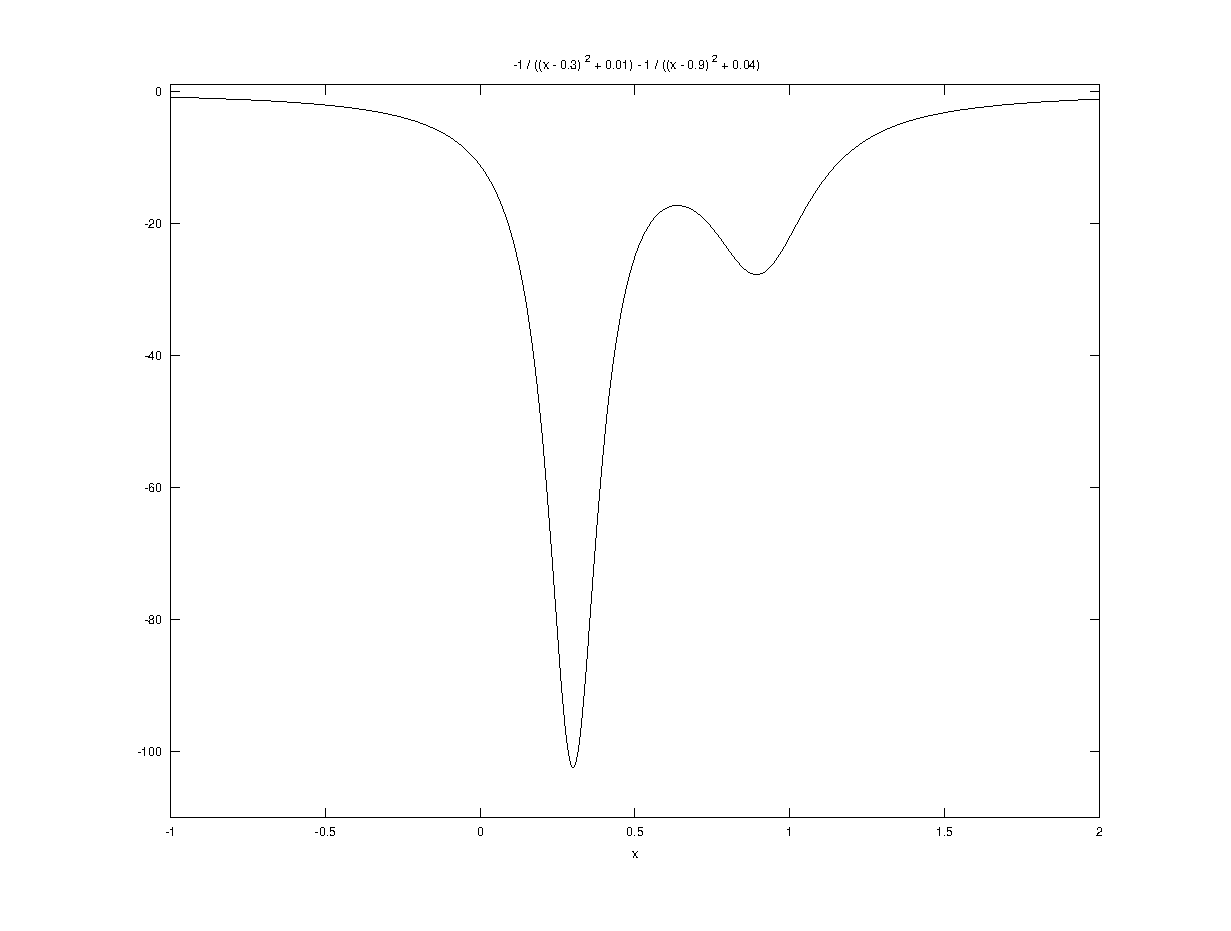
\includegraphics[width=0.6\textwidth]{fmin.eps}
	\end{center}
	
	\begin{enumerate}
		\item[(i)] We use $\left(0,\frac{1}{2}\right)$ as the initial interval.
		\begin{verbatim}
			[a,b] = goldsec(f, 0, 0.5, 1e-8)
			a =  0.300375617070495
			b =  0.300375626326580
		\end{verbatim}
		\begin{align*}
			-f({\text{a}})&= 102.501408560372 \\
			-f({\text{b}})&= 102.501408560372 \\
		\end{align*}
		\item[(ii)] We use $\left(0,\frac{1}{5},\frac{1}{2}\right)$ as the initial bracket for the minimum.
		\begin{verbatim}
			p = parab(f, 0, 0.2, 0.5, 10)
			Columns 1 through 3:
			0.273575619912928   0.335215298966089   0.297714018039367

			Columns 4 through 6:
			0.300794515485728   0.300508503190500   0.300375573369255

			Columns 7 through 9:
			0.300375603984782   0.300375621620731   0.300375621641481

			Column 10:
			0.300375621631106
		\end{verbatim}
		\begin{align*}
			-f({\text{p}}) = 102.501408560372 \\
		\end{align*}
		\item[(iii)] We use $\left(0,\frac{1}{2}\right)$ as the initial interval.
		\begin{verbatim}
			m = fminbnd(f, 0, 0.5)
			m =  0.300375621982956
		\end{verbatim}
		\begin{align*}
			-f({\text{m}}) = 102.501408560372 \\
		\end{align*}
		The graph of $f(x)$ below confirms that its global maximum is approximately 102.5 attained at $x \approx 0.30$. 
		\begin{center}
			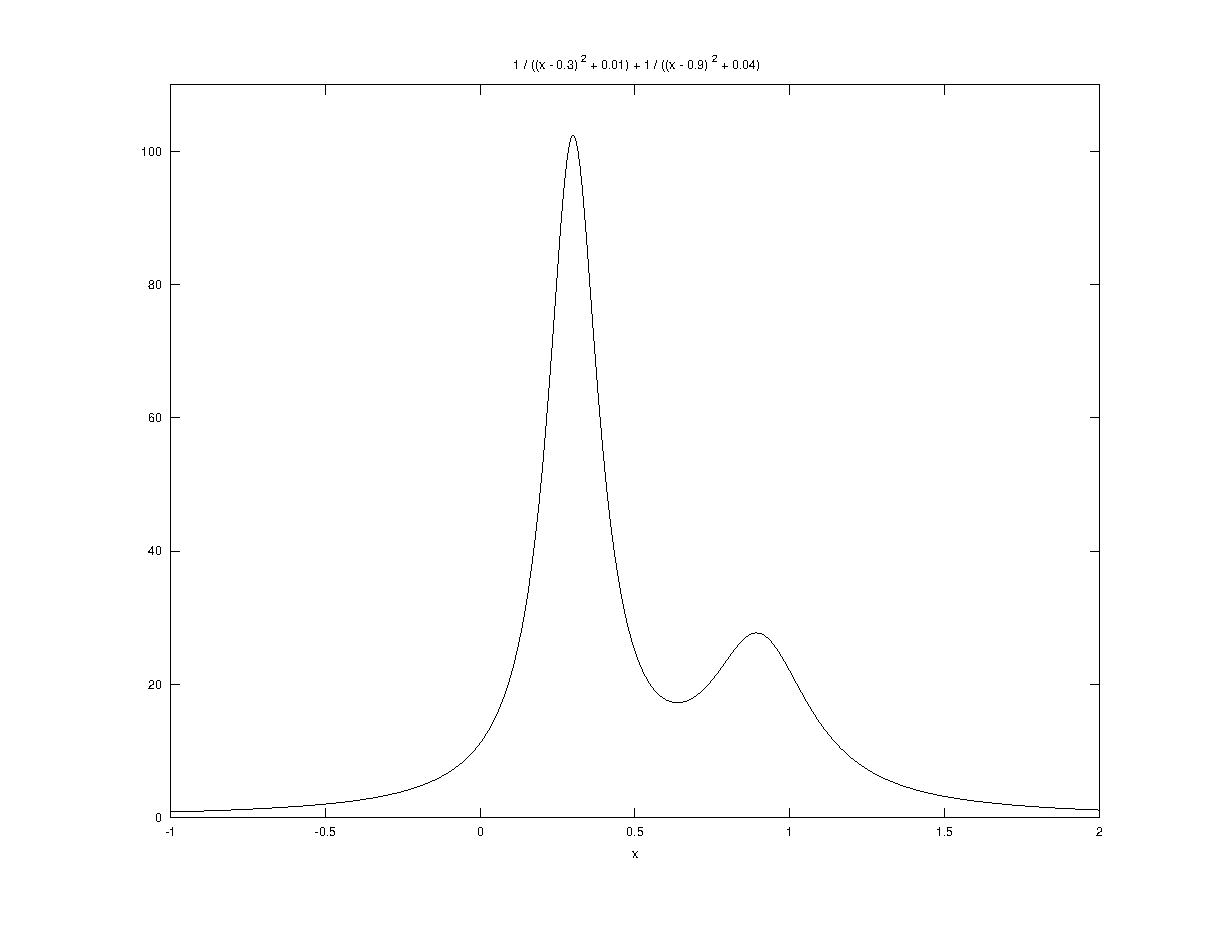
\includegraphics[width=0.6\textwidth]{fmax.eps}
		\end{center}
		
	\end{enumerate}
	\item[(b)] To determine our best estimate, we compare the different function values under each method and check for the largest $-f(x^*)$.
	\begin{align*}
		-f(x_{\text{a}})-(-f(x_{\text{b}}))=0 \ &\Rightarrow \ -f(x_{\text{a}}) = -f(x_{\text{b}}) \\
		-f(x_{\text{p}})-(-f(x_{\text{a}})) \approx 2.1316 \times 10^{-13} \ &\Rightarrow \ -f(x_{\text{p}})> -f(x_{\text{a}})  \\
		-f(x_{\text{m}})-(-f(x_{\text{a}}))  \approx 2.1316 \times 10^{-13} \ &\Rightarrow \ -f(x_{\text{m}}) > -f(x_{\text{a}})  \\
		-f(x_{\text{m}})-(-f(x_{\text{p}}))=0 \ &\Rightarrow \ -f(x_{\text{m}}) = -f(x_{\text{p}}) \\
	\end{align*}
	We conclude that parab and fminbnd provide a better estimate than goldsec. Moreover, there is negligible difference (if any at all) between the former two methods. We estimate the accuracy of each method by evaluating $f''(x^*)$.
	\begin{align*}
		f''(x)&=\frac{8(x-0.9)^2}{\big((x-0.9)^2+0.04\big)^3}+\frac{8(x-0.3)^2}{\big((x-0.3)^2+0.01\big)^3} \\
		&-\frac{2}{\big((x-0.9)^2+0.04\big)^2}-\frac{2}{\big((x-0.3)^2+0.01\big)^2} \\
		f''(x_{\text{p}})&=-19965.73926483396 \\
		f''(x_{\text{m}})&=-19965.73926159880 \\
	\end{align*}
	Analysis of rounding errors show that parab has greater accuracy than fminbnd since $\Delta x_{\text{p}} < \Delta x_{\text{m}}$.
	$$\Delta x_{\text{p}}=\sqrt{\frac{2\varepsilon_{\text{mach}}}{|f''(x_{\text{p}})|}}=1.49139407334926 \times 10^{-10}$$
	$$\Delta x_{\text{m}}=\sqrt{\frac{2\varepsilon_{\text{mach}}}{|f''(x_{\text{m}})|}}=1.49139407347009 \times 10^{-10}$$
	Thus, successive parabolic interpolation gives the best estimate for finding the maximum of $f(x)$.
\end{enumerate}

\subsubsection*{Question 6}
We express the relationship between the angle $\alpha$ and distance $x$ by the following implicit function.
$$f(x,\alpha)=0.0122583125x^2-x\sin\alpha\cos\alpha+13\cos^2\alpha=0$$
To find the maximum distance $x$ at which the target can be reached, we define $x=g(\alpha)$ where $g$ takes a value of $\alpha$ and returns $x$ as the larger root of $f(x,\alpha)$. We then determine the range of $\alpha$ for which $f(x,\alpha)$ has real roots to know where $g(\alpha)$ is defined. Using an iterative loop to compute the roots of each polynomial generated and disregarding any complex roots, we find the maximum distance $x \approx 24.56$ metres.

\pagebreak

\textbf{Appendix}

\begin{enumerate}

	\item 
	\begin{verbatim}
		function y=wave(x)
			y=sin(10*x)-x;
		endfunction
		
		x=linspace(-1,1,201);
		plot(x,wave(x))
		hold on 
		plot([-1 1],[0 0])
		print('wave.eps','-deps')

		fzero(@wave,[-1,-0.8])
		fzero(@wave,[-0.8,-0.5])
		fzero(@wave,[-0.5,-0.1])
		fzero(@wave,[-0.1,0.1])
		fzero(@wave,[0.1,0.5])
		fzero(@wave,[0.5,0.8])
		fzero(@wave,[0.8,1])
	\end{verbatim}
	
	\item
	\begin{verbatim}
		function y=tangent(x)
		y=x-tan(x);
		endfunction
		
		fzero(@tangent,[1000000*pi,1000000.5*pi])
	\end{verbatim}
	
	\item
	\begin{verbatim}
		function x=iterate(g,x0,n)
			x=zeros(1,n+1);
			x(1)=x0;
			for i=1:n
				x(i+1)=g(x(i));
			end
		endfunction
		
		function y=gone(x)
			y=(x.^2+2)/3;
		endfunction
		
		x1=iterate(@gone,1.9,100)
		x1=iterate(@gone,2.1,100)
		
		function y=gtwo(x)
			y=sqrt(3*x-2);
		endfunction
		
		x2=iterate(@gtwo,1.9,50)
		err2=abs(x2-2);
		ratio2=err2(2:51)./err2(1:50)
		
		function y=gthree(x)
			y=3-2./x;
		endfunction
		
		x3=iterate(@gthree,1.9,50)
		err3=abs(x3-2);
		ratio3=err3(2:50)./err3(1:49)
		
		function y=gfour(x)
			y=(x.^2-2)/(2*x-3);
		endfunction
		
		x4=iterate(@gfour,1.9,5)
		err4=abs(x4-2);
		ratio4=err4(2:6)./err4(1:5)
	\end{verbatim}
	
	\item
	\begin{enumerate}
		\item
		\begin{verbatim}
			reciprocal(0.9,20)
			Columns 1 through 6:
			0.90000   0.18000   0.29520   0.41611   0.48593   0.49960   

			Columns 7 through 13:
			0.50000   0.50000   0.50000   0.50000   0.50000   0.50000 
		\end{verbatim}
		
		\item
		\begin{enumerate}
		
			\item[(i)]
			\begin{verbatim}
				reciprocal(1.01,20)
				Columns 1 through 4:
				1.0100e+000   -2.0200e-002   -4.1216e-002   -8.5830e-002  
					
				Columns 14 through 17:
				-1.4177e+070   -4.0196e+140   -3.2315e+281   -Inf
					
				reciprocal(-0.99,20)
				Columns 1 through 4:
				-9.9000e-001   -3.9402e+000   -3.8931e+001   -3.1091e+003
					
				Columns 8 through 11:
				-2.5041e+060   -1.2541e+121   -3.1456e+242    -Inf
				\end{verbatim}
				
			\item[(ii)]
			\begin{verbatim}
				reciprocal(0.999999999999999944499191,10)
				1   0   0   0   0   0   0   0   0   0   0
			\end{verbatim}
			
			\pagebreak
			
			\item[(iii)]
			\begin{verbatim}
				reciprocal(0.99999999999999994449919099999,60)
				Columns 1 through 4:
				1.0000e+000  2.2204e-016  4.4409e-016  8.8818e-016
				
				Columns 51 through 54:
				1.1060e-001  1.9673e-001  3.1606e-001  4.3233e-001   

				Columns 55 through 59:
				4.9084e-001  4.9983e-001  5.0000e-001  5.0000e-001
			\end{verbatim}
		\end{enumerate}
	\end{enumerate}
	
	\item
	\begin{enumerate}
		\item
			\begin{verbatim}
				f=@(x) -1./((x-0.3).^2+0.01)-1./((x-0.9).^2+0.04);
				ezplot(f,[-1,2])
				axis([-1 2 -110 1])
				print('goldsec.eps','-deps')
			\end{verbatim}
		\item
			\begin{verbatim}
				d2f=@(x) (8.*(x-.9).^2)./((x-.9).^2+.04).^3 
				+ (8.*(x-.3).^2)./((x-.3).^2+.01).^3 
				- 2./((x-.9).^2+.04).^2 - 2./((x-.3).^2+.01).^2
				
				d2fp=d2f(p(10));
				rp=sqrt(2*eps/abs(d2fp))
				rm=sqrt(2*eps/abs(d2f(m)))
			\end{verbatim}
	\end{enumerate}
	
	\item
	\begin{verbatim}
		a=linspace(0,pi/2,100)';
		c=9.80665/800;
		p=[c*ones(length(a),1) -sin(a).*cos(a) 13*cos(a).^2];
		pr=zeros(length(a),2);  
		maxpr=zeros(length(a),1);  

		for i=1:length(a)
		pr(i,1:2)=roots(p(i,:));
		maxpr(i)=max(pr(i,1:2));
		xmax=max(real(maxrp))
		end

		xmax
	\end{verbatim}
	
\end{enumerate}

\end{document}